\section{Evaluation Strategy} \label{sec:evaluation-strategy}

This section begins with a discussion of the evaluation requirements and challenges.
Then, it introduces the proposed evaluation strategy and explains the rationale behind its design.
Finally, each step of the evaluation process is described in detail.

\subsubsection*{Evaluation Requirements}

The evaluation strategy must satisfy the following conditions:

\begin{itemize}
    \item It must have the capacity to address \textbf{\ac{RT} 3} and \textbf{\ac{RT} 4} in a comprehensive manner.
          This includes the ability to determine the optimal parameters for the Citation Recommender, the Language Recommender, as well as the best hybridization order.
    \item The results should be objective and reproducible.
          To achieve this, the evaluation must be systematic, data-driven, and independent of any prior knowledge.
    \item The process must be computationally manageable considering the available resources and time constraints.
\end{itemize}

To set the stage and clarify the rationale behind our assessment method, we first describe the straightforward but computationally infeasible approach.
The simplest way to evaluate the Hybrid Recommender's performance is to conduct an exhaustive grid search over all conceivable input combinations.
More specifically, we would need to: (i) construct an evaluation dataset where each row corresponds to a combination of query paper from the base dataset, all possible feature weights, and all available language models, (ii) conduct one inference call for each row, and (iii) calculate the \ac{AP} for each candidate and final ranking.
Those feature weights and language models yielding the highest \ac{MAP} scores across all inference runs are selected as the optimal parameters.

This approach encounters both computational and conceptual challenges:

\begin{enumerate}
    \item The feature weights are numerically unbounded since each weight can be set to any real non-negative value. Thus, there are infinitely many combinations of feature weights we would need to evaluate.
          Further, even a large finite subset of feature weights may render the search space too large to make an exhaustive grid search computationally feasible.
    \item Using query documents from the \emph{readnext} dataset for inference only allows the assessment of in-sample performance for seen documents.
          Evaluating the generalization performance for new and unseen query papers is not possible with this approach.
          However, inference for unseen query papers is the primary use case of the recommender system, particularly in the long run with more and more papers being published in the future.
          Thus, quantifying the generalization performance is essential.
\end{enumerate}

\subsubsection*{Proposed Evaluation Strategy}

To overcome the aforementioned challenges, this thesis' evaluation strategy incorporates the following components:

\begin{enumerate}
    \item \textbf{Randomized Search for Feature Weights}: Instead of an exhaustive grid search, a randomized search is utilized for the feature weights. The search space is confined to non-negative integer values to enhance the interpretability of the weight vectors.
    \item \textbf{Data Splitting}: A traditional random split of the data into training, validation, and test sets is adopted. The split ratio is set such that the training set includes $80\%$, and the validation and test sets each contain $10\%$ of the data. With a total of $10,000$ documents in the \emph{readnext} corpus, this results in $8,000$ documents for training and $1,000$ documents for validation and testing, respectively. Note that this split is only relevant for the evaluation process. When using the recommender system for inference, recommendations can be drawn from the entire corpus of $10,000$ documents.
    \item \textbf{Training Set}: The training set serves two purposes. First, it is used to train the keyword-based language models TF-IDF and BM25 with all remaining models being used in their pretrained form.
          Second, all candidate papers, and thus all potential recommendations, are drawn from the training set.
    \item \textbf{Validation Set}: The validation set is employed to conduct the randomized search for the best feature weights of the Citation Recommender. This includes both finding appropriate ranges for the feature weights as well as specific candidate weight vectors within these ranges.
    \item \textbf{Test Set}: The final performance evaluation that all results presented in \Cref{sec:evaluation-results} are based on is conducted on a separate test set.
          This separation ensures an unbiased assessment of the generalization performance for new and unseen query papers.
\end{enumerate}

The subsequent section elaborates on the three-step data-driven evaluation strategy of this thesis, visualized in \Cref{fig:evaluation-strategy} and \Cref{fig:evaluation}.
The number of sampled feature weight vectors ($n$), sampled input combinations ($N$), and selected candidates ($k$) are chosen to balance computational feasibility with statistical validity.
Generally, higher values for $n$, $N$, and $k$ lead to more accurate results but in return increase the computational complexity of the evaluation process.

\begin{figure}[htb!]
    \centering
    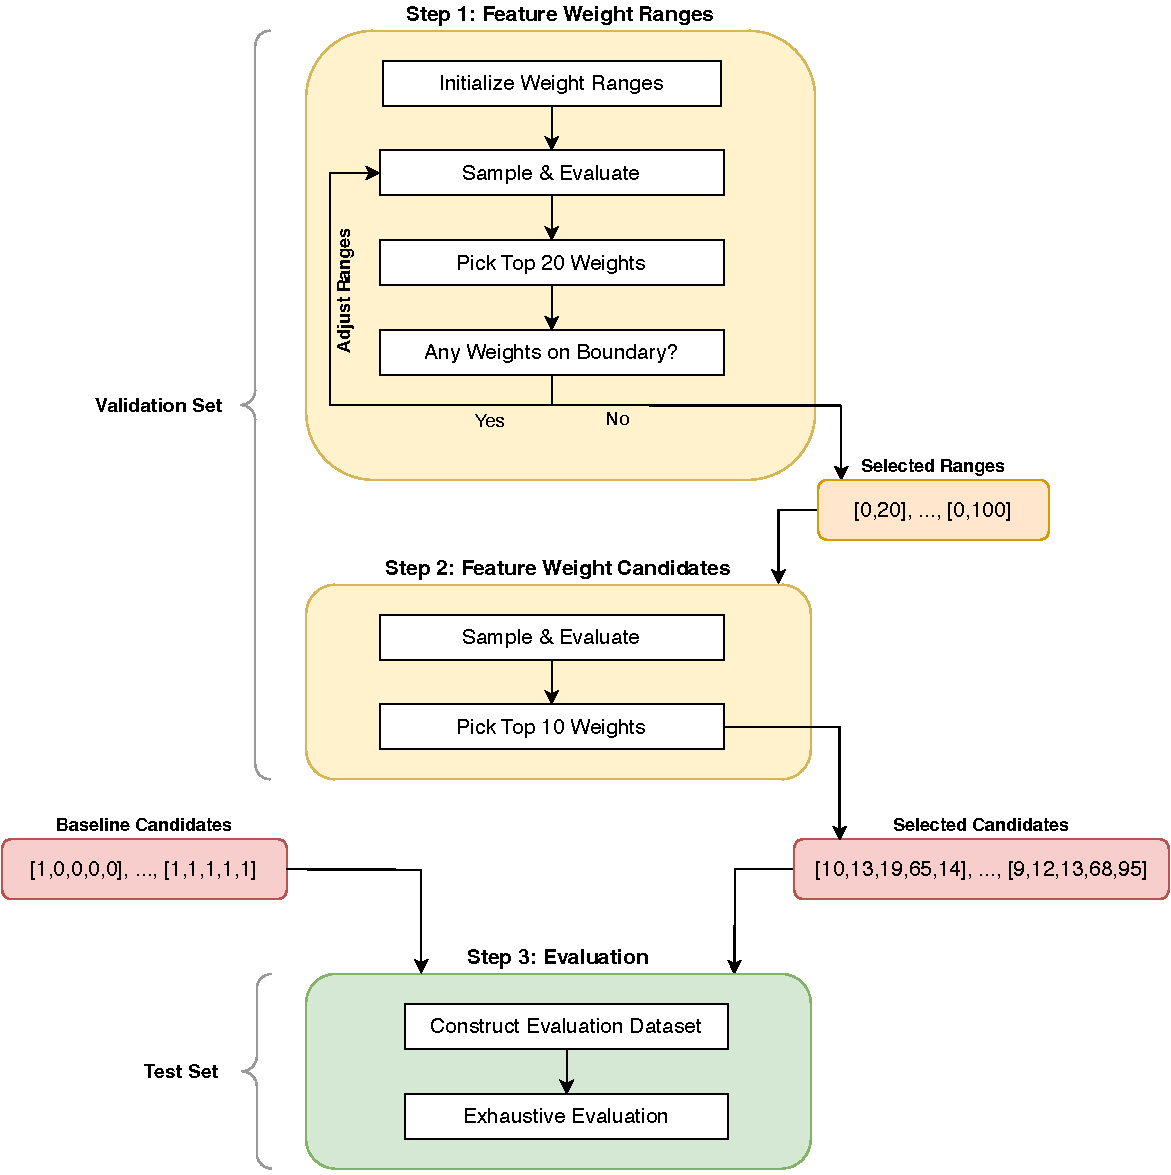
\includegraphics[width=0.8\textwidth]{diagrams/evaluation_strategy.pdf}
    \caption[Evaluation Strategy]{Evaluation Strategy. The evaluation strategy consists of three steps. The first two steps - finding suitable feature weight ranges and specific candidate weight vectors from those ranges - are performed on the validation set.
        The top ten candidates and six baseline weight vectors are used in the final step to construct the evaluation dataset and measure the performance of the Hybrid Recommender on the test set.}
    \label{fig:evaluation-strategy}
\end{figure}


\subsubsection*{Step 1: Finding Feature Weight Ranges}

The first step aims to identify appropriate ranges for the feature weights of the Citation Recommender on the validation set.
Its goal is to discover ranges that are neither too narrow nor too wide. Both extremes lead to suboptimal results:
Overly narrow ranges lead to a highly restricted search space, which may exclude the optimal feature weights.
Conversely, overly wide ranges may render the process computationally intractable. Further, the selected weights from a very broad search space may still be far from the optimal weights.

The iterative search proceeds as follows:

\begin{enumerate}
    \item Initialize all feature weight ranges with the integer interval $[0, 5]$.
    \item Sample $n=50$ random weight vectors and construct all combinations with the $1000$ query documents in the validation set and the $8$ language models, yielding an input space of $400,000$ values.
    \item Randomly sample $N=1000$ input combinations, ensuring an average of $20$ samples for each weight vector.
          Compute the marginal \ac{MAP} for all weight vectors, averaged over all query documents and language models, and analyze the $20$ top-performing candidates.
          If any weight within those vectors is at the boundaries of the current ranges, the ranges are expanded, as the optimal weights might lie outside the current ranges.
          Subsequently, the sampling and evaluation steps are repeated with the adjusted ranges.
          Conversely, if none of the weights are at the boundaries, the current ranges are deemed appropriate and the process moves to step 2.
\end{enumerate}


\subsubsection*{Step 2: Randomized Feature Weights Search}

The second step, conducted on the validation set, assesses a larger number of feature weights within the ranges selected in step 1 and identifies the top $k=10$ best-performing weight vectors.

This step is performed as follows:

\begin{enumerate}
    \item Sample $n=200$ feature weight combinations from the identified ranges of step 1, resulting in $1,600,000$ input combinations, accounting for the $8$ language models and $1000$ query documents of the validation set.
    \item Randomly select $N=10,000$ combinations, ensuring an average of $50$ samples for each weight vector.
    \item Similar to step 1, compute the marginal \ac{MAP} for the weight vectors, averaged over all query documents and language models, and select the top $k=10$ candidates for the final evaluation in step 3.
\end{enumerate}

Since step 2 does not operate sequentially like the first step, the process can be parallelized for more efficient computation.


\subsubsection*{Step 3: Performance Evaluation}

The third step evaluates the inference performance of various input combinations on the test set.

The evaluation procedure is as follows:

\begin{enumerate}
    \item Augment the selected feature weights of step 2 with the $6$ baseline weight vectors $[1, 0, 0, 0, 0], [0, 1, 0, 0, 0], \ldots, [0, 0, 0, 0, 1], [1, 1, 1, 1, 1]$ resulting in $k=16$ candidates.
          These simple weight combinations are added for interpretability: Each unit weight vector isolates the effect of a single feature while the vector of ones contributes the same impact to each of the five features.
          Coupled with the $8$ language models and $1000$ query documents of the test set, the evaluation dataset comprises $128,000$ combinations.
    \item Unlike previous steps, the evaluation is exhaustive without any prior subsampling. Inference runs for each of the $128,000$ input combinations are initiated.
          The resulting candidate and final recommendation rankings are evaluated using the \ac{MAP} and the measure for recommendation diversity as defined in \Cref{sec:arxiv-labels}.
\end{enumerate}

Similar to the second step, step 3 can be parallelized for efficient computation. \Cref{fig:evaluation} visualizes the third and final component of the evaluation process.

\begin{figure}[htb!]
    \centering
    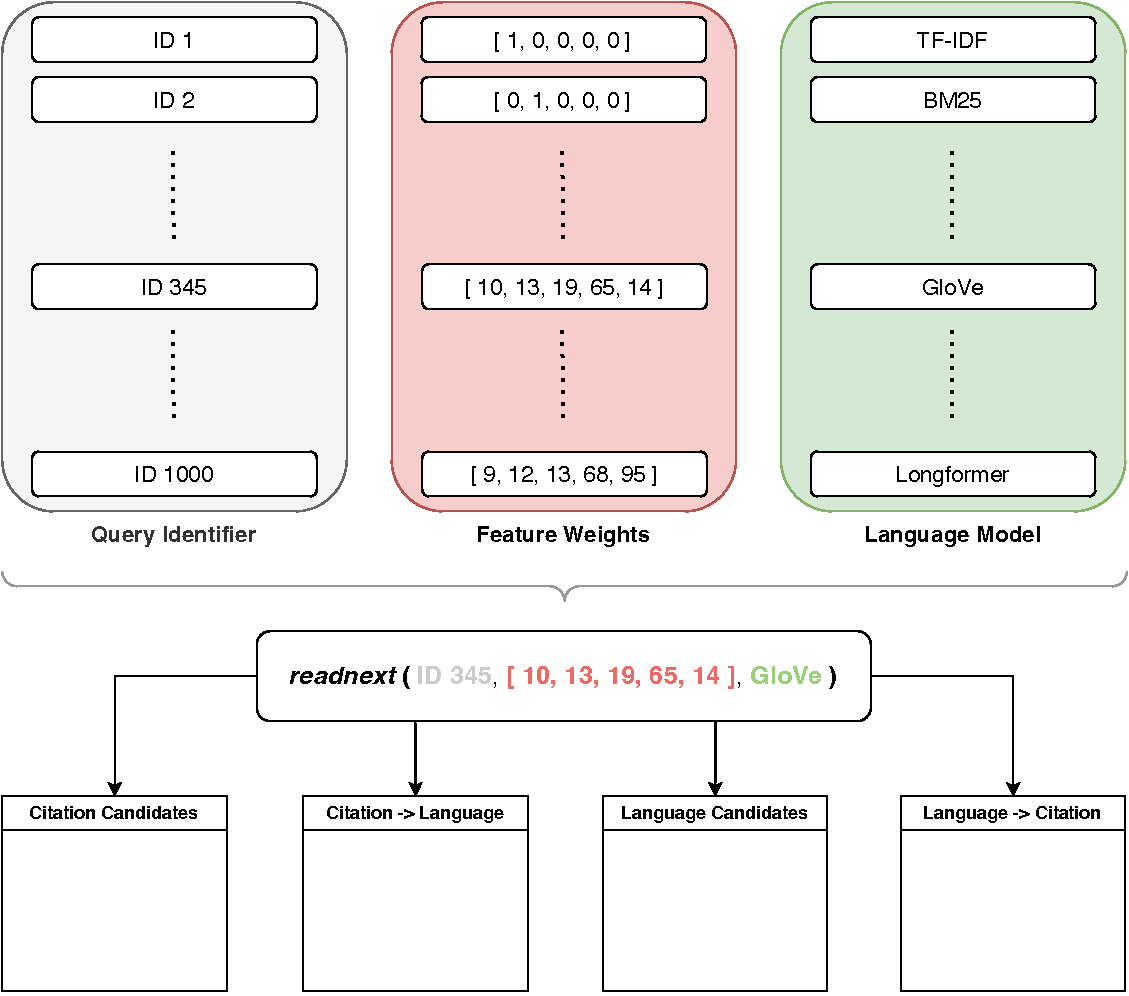
\includegraphics[width=0.9\textwidth]{diagrams/evaluation.pdf}
    \caption[Evaluation]{Evaluation of the Hybrid Recommender. The evaluation dataset is constructed from each combination of the $1,000$ test set query papers, $16$ feature weights, and $8$ language models, resulting in $128,000$ rows. One inference run is conducted for each row, returning recommendation lists of the Citation Recommender candidates, the Language Recommender candidates, and final rankings of the \ac{C2L} and the \ac{L2C} Hybrid Recommenders. All recommendation rankings are evaluated using the \ac{MAP} and the measure for recommendation diversity.
    }
    \label{fig:evaluation}
\end{figure}


\subsubsection*{Discussion}

The proposed three-step evaluation strategy has several advantages.
It is systematic and reproducible, data-driven, and computationally feasible.
However, it also has some drawbacks.
In reference to step 1, the range of a given feature expands as soon as its corresponding weight reaches the interval boundary for \emph{any} of the 20 top-performing weight vectors.
This conservative approach may lead to overly broad feature weight ranges.
Moreover, range adjustments may not lead to improved candidates in the first place, as a weight vector may perform well \emph{despite} one of its values being at the interval boundaries, not \emph{because} of it.

One way to address this shortcoming is to require a minimum number of weights at the boundary before expanding the range.
Alternatively, the process of adjusting the ranges could be bidirectional by iteratively making the ranges smaller and larger until the optimal ranges are found.
However, to maintain the evaluation strategy's simplicity and clarity, we opted against these modifications.
